\chapter{AlphaFold-disorder (SASA): Development of Procedures}
\label{chp:development}
In this chapter we will talk about the actual development part of the thesis. We worked on three procedures:
\begin{itemize}
    \item \textbf{Detection of secondary structure using protein atomic coordinates}: development of a procedure that assigns to each residue its secondary structure. It's based on P-SEA algorithm, described in this scientific paper\cite{psea};
    \item \textbf{Computation of RSA, using Shrake-Rupley algorithm}: We calculated SASA using Shrake-Rupley algorithm and then computed RSA with normalization factors;
    \item \textbf{Implementation of FoldComp library}: for reading protein files in .fcz, which is a compression of .pdb files.
\end{itemize}
Let's analyse the process of development for each of these procedure.

\section{Secondary Structure Detection with Protein Atomic Coordinates}
In the scientific paper of P-SEA, the researchers suggest an algorithm based on protein atomic coordinates of the central carbon atom of the residue, the alpha Carbon.  

For each residue i, we want to calculate these distance measures:
\begin{itemize}
    \item d2i: it's the distance between the residue (i-1) and the residue (i+1);
    \item d3i: it's the distance between the residue (i-1) and the residue (i+2);
    \item d4i: it's the distance between the residue (i-1) and the residue (i+3);
\end{itemize}

And these angle measures:
\begin{itemize}
    \item $\tau$i: the angle formed by the residues (i-1), i and (i+1);
    \item $\alpha$i: the dihedral angle formed by the residues (i-1), i, (i+1) and (i+2).
\end{itemize}

Specific range of values in d2, d3, d4, $\tau$i, $\alpha$i determine in which secondary structure that residue falls into, among the main three categories:
\begin{itemize}
    \item \textbf{Helices};
    \item \textbf{Strands}: such as beta-sheets parallel and anti-parallel;
    \item \textbf{Coils}: turns and loops;
\end{itemize}

The thresholds for belonging in one of the two non coil secondary structure are shown in the table \ref{tab:thr-psea}.

\begin{table}[h!]
    \centering
    \begin{tabular}{|c|c|c|}
    \hline
        Parameters & Helix & Strand \\
    \hline
        Angle $\tau$ (\textdegree) & 89\hspace{0.3em} $\pm$\hspace{0.3em} 12 & 124\hspace{0.3em} $\pm$\hspace{0.3em} 14 \\
        Dihedral angle $\alpha$ (\textdegree) & 50\hspace{0.3em} $\pm$\hspace{0.3em} 20 & -170\hspace{0.3em} $\pm$\hspace{0.3em} 45 \\
        & & \\
        Distance d2 (\AA) & 5.5\hspace{0.3em} $\pm$\hspace{0.3em} 0.5 & 6.7\hspace{0.3em} $\pm$ \hspace{0.3em} 0.6\\
        Distance d3 (\AA) & 5.3\hspace{0.3em} $\pm$ \hspace{0.3em} 0.5 & 9.9\hspace{0.3em} $\pm$ 0.9 \\
        Distance d4 (\AA) & 6.4\hspace{0.3em} $\pm$ \hspace{0.3em} 0.6 & 12.4\hspace{0.3em} $\pm$ \hspace{0.3em} 1.1\\
        \hline
    \end{tabular}
    \caption{Parameters for P-SEA assignment of secondary structure.}
    \label{tab:thr-psea}
\end{table}

\begin{figure}[h!]
    \centering
    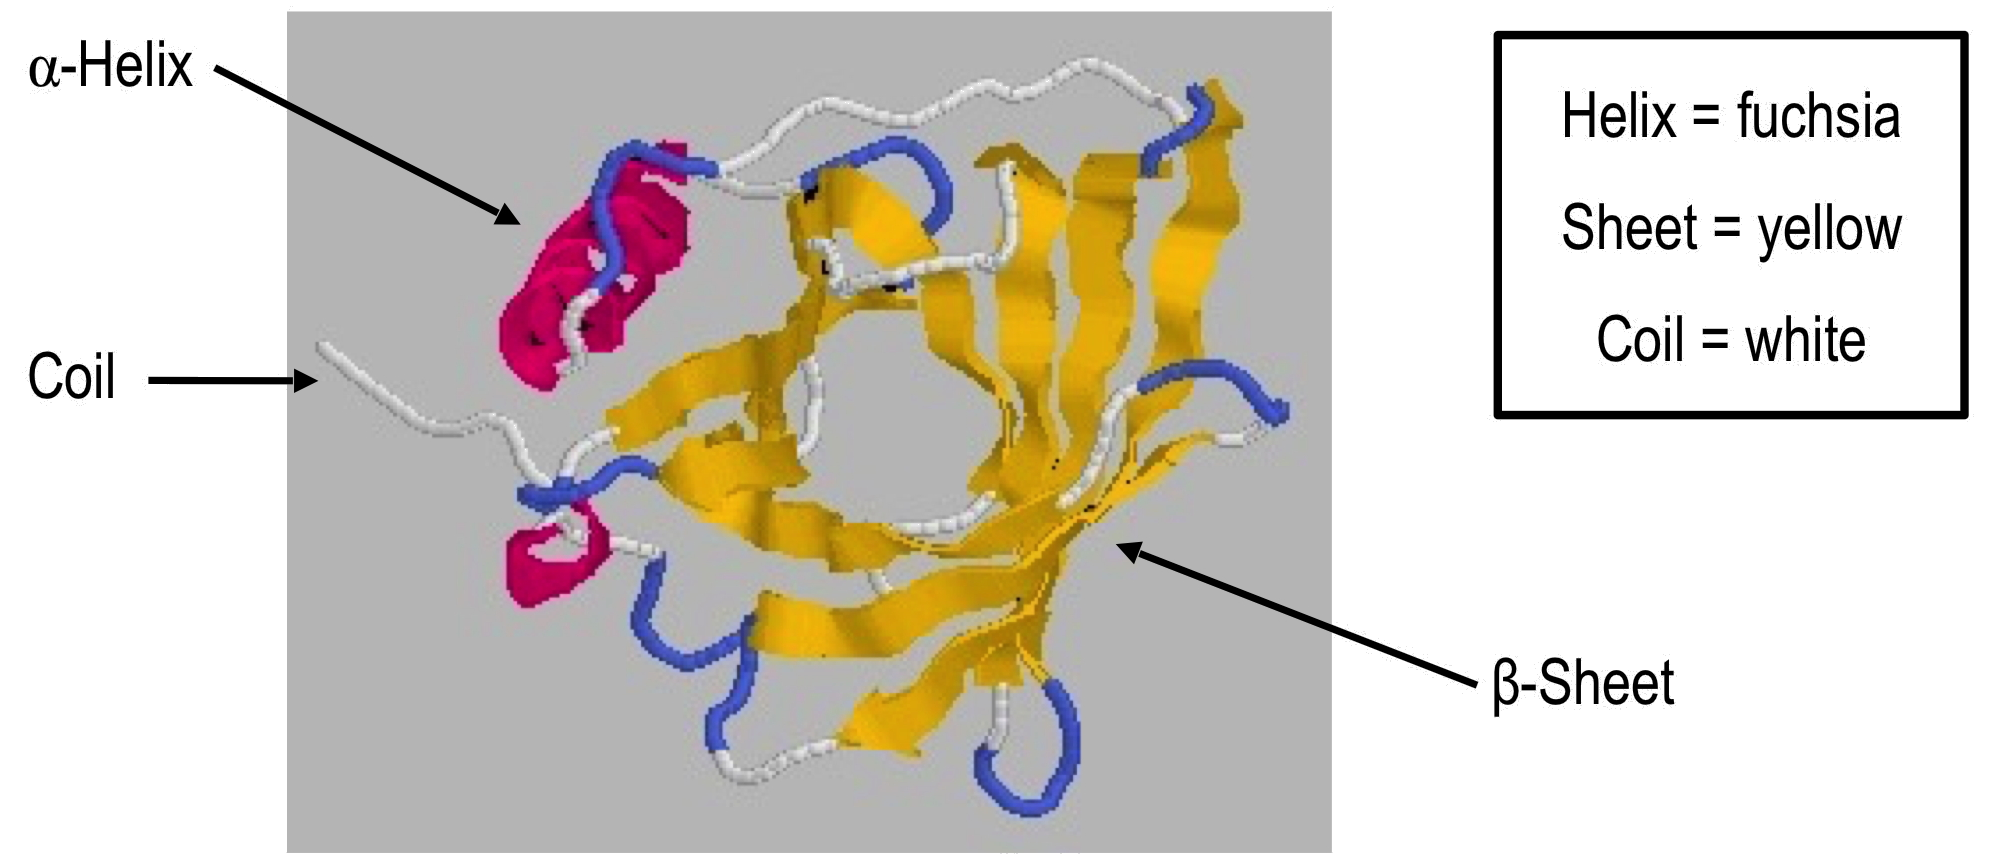
\includegraphics{res/dev/coil.png}
    \caption{The threee secondary structure P-SEA can identify}
\end{figure}

Let's see how we implemented the idea of algorithm discussed on the paper\cite{psea}.
\subsection{Algorithm}

\section{Computation of RSA with Shrake-Rupley Algorithm}
\section{Implementation of FoldComp Library}
